\documentclass[fleqn]{article}
\oddsidemargin 0.0in
\textwidth 6.0in
\thispagestyle{empty}
\usepackage{import}
\usepackage{amsmath}
\usepackage{graphicx}
\usepackage{flexisym}
\usepackage{calligra}
\usepackage{amssymb}
\usepackage{bigints} 
\usepackage[english]{babel}
\usepackage[utf8x]{inputenc}
\usepackage{float}
\usepackage[colorinlistoftodos]{todonotes}


\DeclareMathAlphabet{\mathcalligra}{T1}{calligra}{m}{n}
\DeclareFontShape{T1}{calligra}{m}{n}{<->s*[2.2]callig15}{}
\newcommand{\scriptr}{\mathcalligra{r}\,}
\newcommand{\boldscriptr}{\pmb{\mathcalligra{r}}\,}

\definecolor{hwColor}{HTML}{1a0252}

\begin{document}

  \begin{titlepage}

    \newcommand{\HRule}{\rule{\linewidth}{0.5mm}}

    \center

    \begin{center}
      
\includegraphics[height=11cm, width=11cm]{asu.png}
    \end{center}

    \vline

    \textsc{\LARGE Quantum Physics II}\\[1.5cm]

    \HRule \\[0.5cm]
    { \huge \bfseries Problem Set One}\\[0.4cm] 
    \HRule \\[1.0cm]

    \textbf{Behnam Amiri}

    \bigbreak

    \textbf{Prof: Onur Erten}

    \bigbreak

    \textbf{{\large \today}\\[2cm]}

    \vfill

  \end{titlepage}

  \begin{enumerate}
    \item \textbf{2-9}

    \begin{center}
      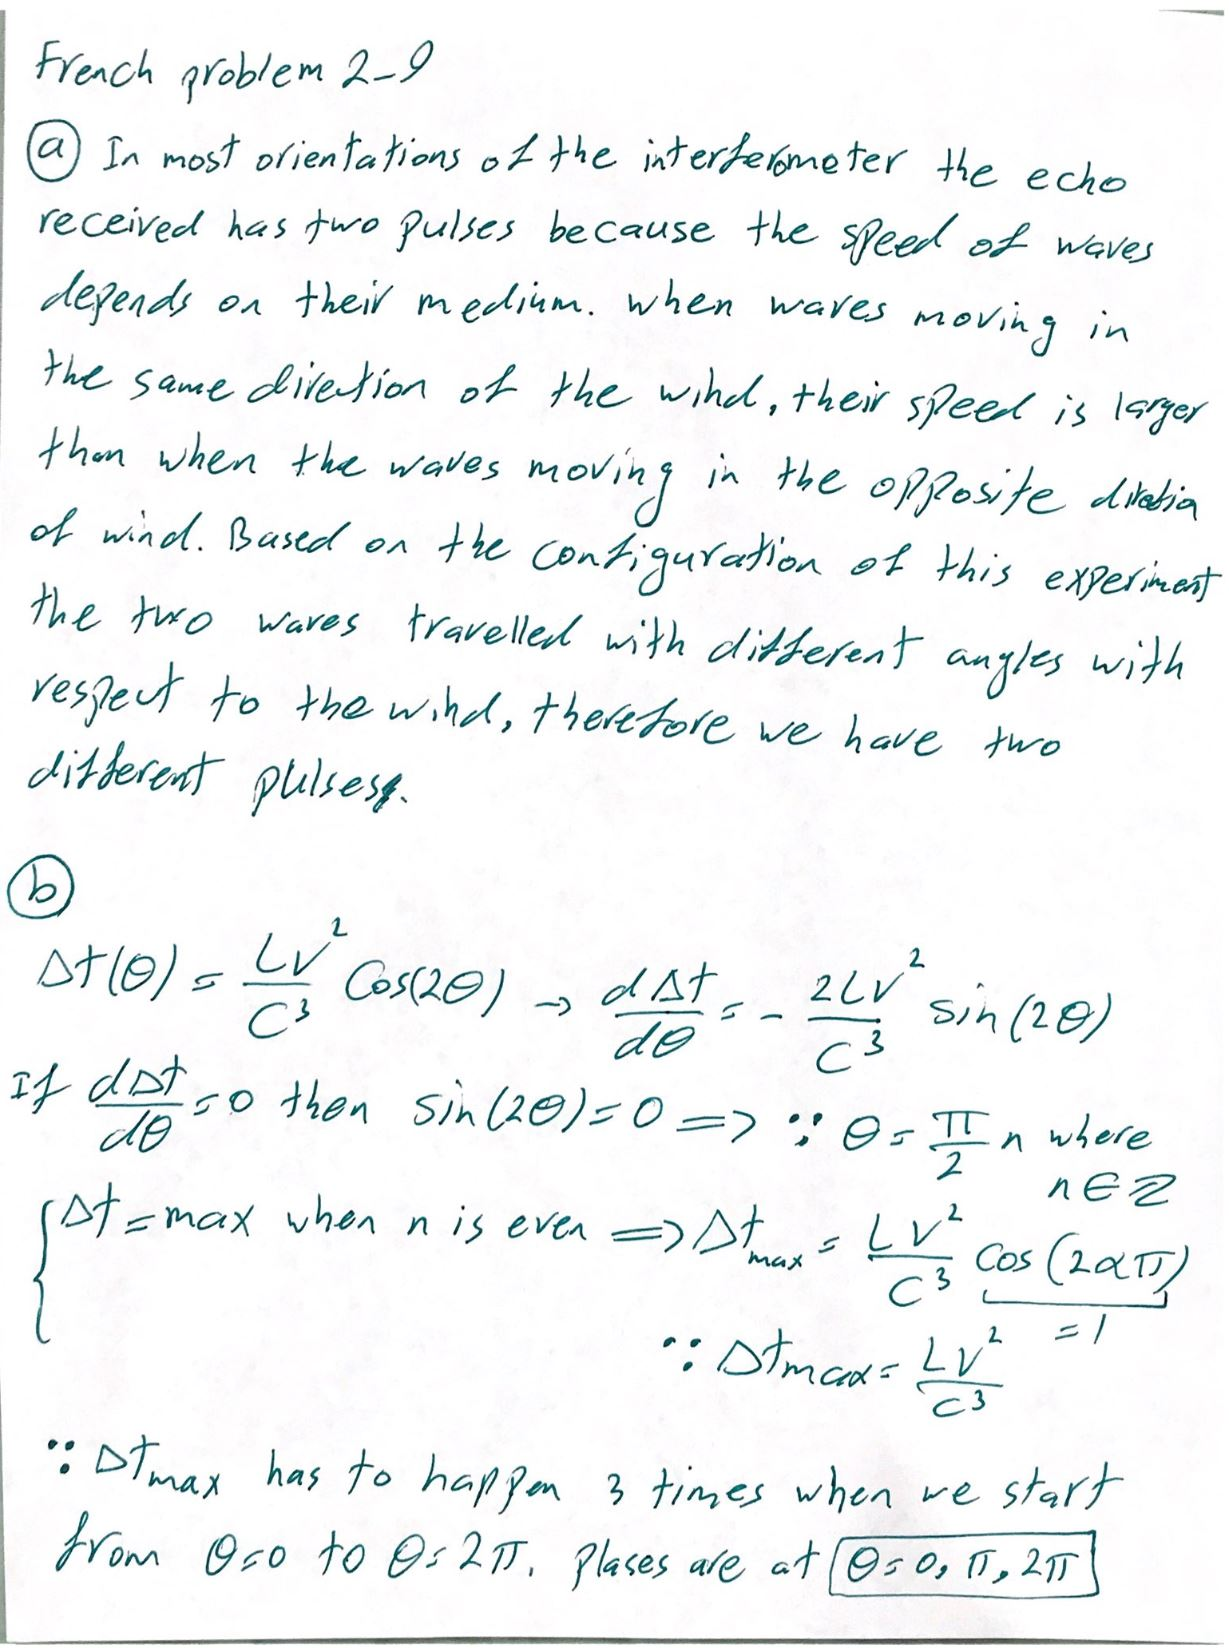
\includegraphics[height=18cm, width=14cm]{2-9A.JPG}
    \end{center}

    \pagebreak

    \begin{center}
      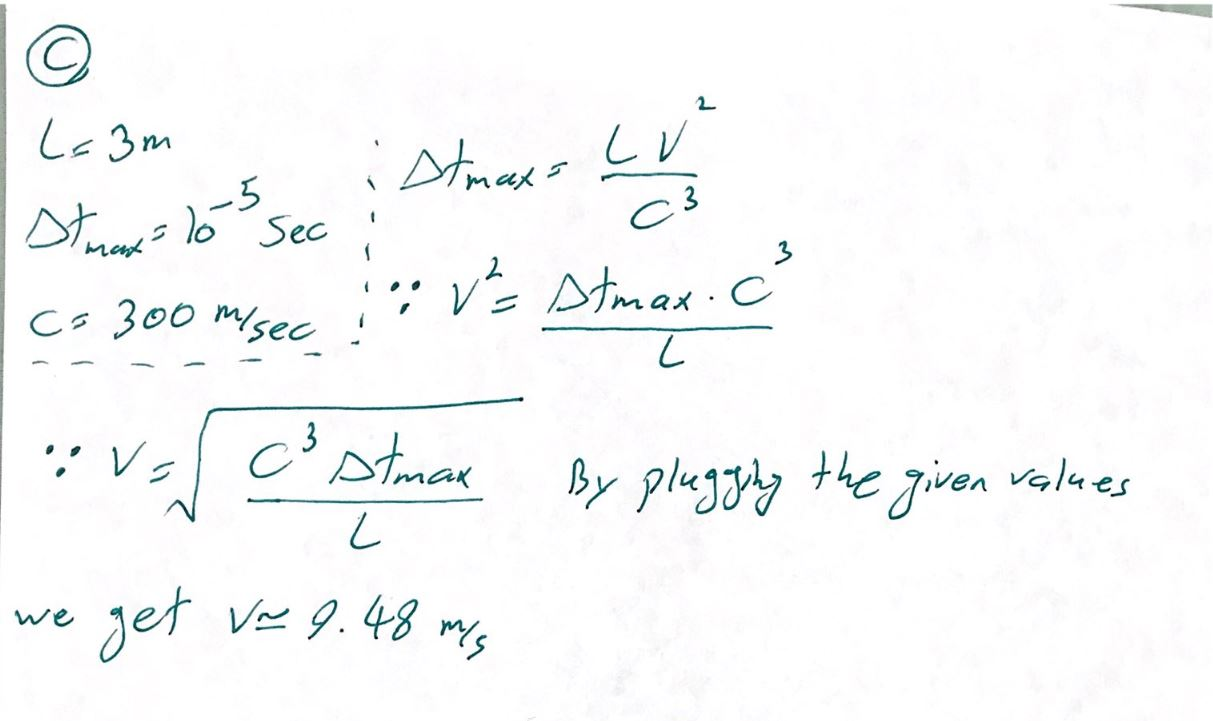
\includegraphics[height=10cm, width=14cm]{2-9B.JPG}
    \end{center}

    \pagebreak

    \item \textbf{4-1}
    
    \begin{center}
      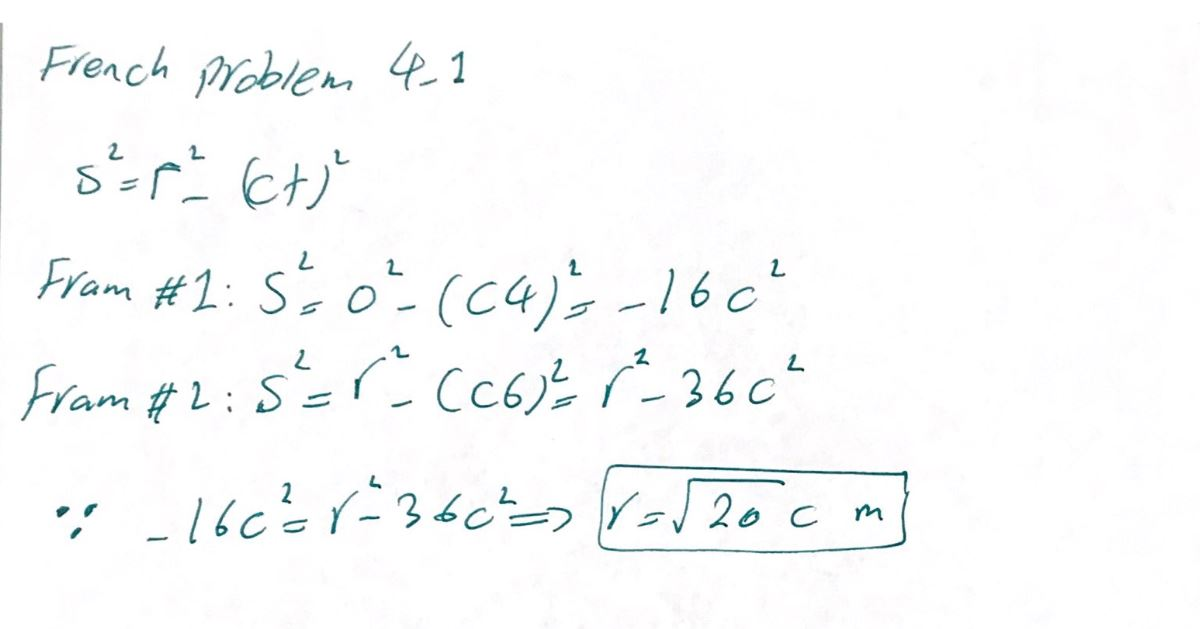
\includegraphics[height=10cm, width=14cm]{4-1.JPG}
    \end{center}

    \pagebreak

    \item \textbf{4-6}
    
    \begin{center}
      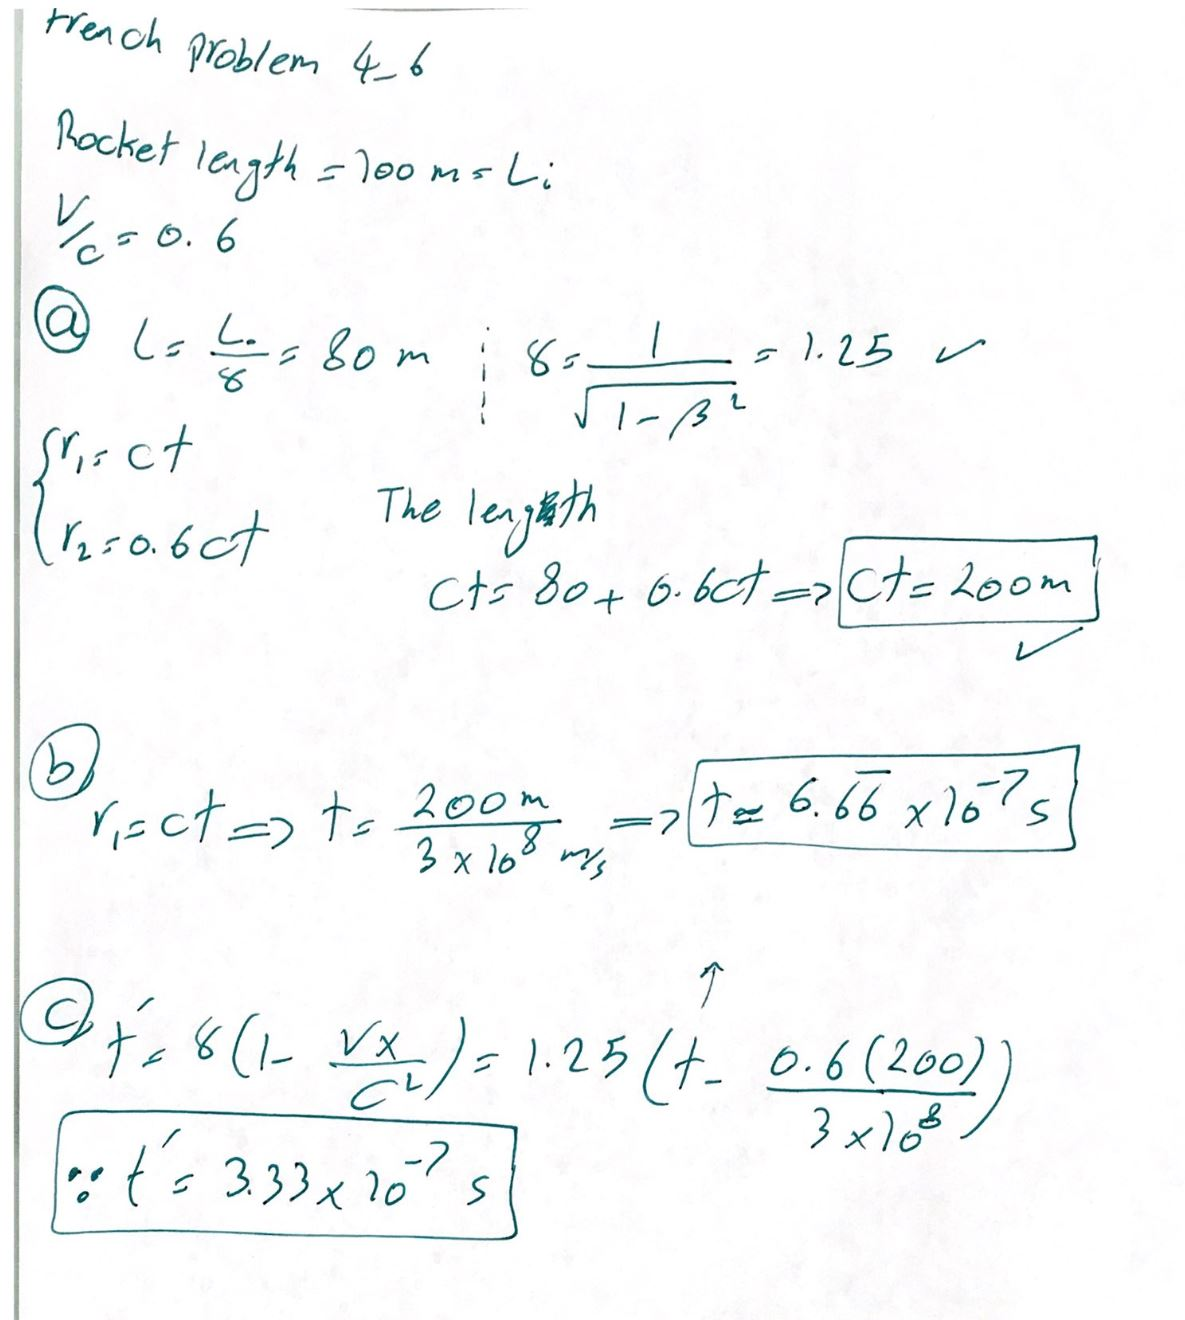
\includegraphics[height=18cm, width=14cm]{4-6.JPG}
    \end{center}


  \end{enumerate}

\end{document}
